% !TEX root = ../msimplicial.tex

\section{Multisimplicial algebra}

\anibal{Write something here}

\subsection{Multisimplicial chains}

The functor of (normalized) \textit{chains} is the composition
\[
\chains \colon \mSet \xra{\bars{-}} \CW \xra{\gchains} \Ch
\]
of the geometric realization and functor of cellular chains.
It can also be described up to natural equivalence as the Yoneda extension of the functor defined on representable objects by
\[
\chains \big( \simplex^{n_1, \dots, n_k} \big) =
\chains(\simplex^{n_1}) \ot \dotsb \ot \chains(\simplex^{n_k}).
\]
The functor of \textit{cochains} is defined using linear duality.

Explicitly, for a $k$-fold multisimplicial set $X$ the $\k$-module $\chains(X)_n$ is freely generated by the non-degenerate $(n_1, \dots, n_k)$-multisimplices $x$ with $n_1 + \dots + n_k = n$ and the differential has the form
\[
d(x) = \sum_{j=1}^k \sum_{\ell_j=1}^{n_j}
(-1)^{n_{1}+\dots+n_{j-1}+\ell_j} \, d^j_{\ell_j}(x).
\]

If we do not mod out by degenerate multisimplices the same formula defines the functor of \textit{non-normalized chains}.
A slight generalization of the classical normalization theorem by MacLane \cite{MacLane} shows that the natural projection between these is a natural chain homotopy equivalence.

\subsection{Chain comparison} \label{ss:comparison chain maps}

Let $X$ be a multisimplicial set and $Y$ a simplicial set.
The Eilenberg--Zilber and Cartan--Serre comparison maps induce natural quasi-isomorphism
\[
\begin{split}
	\EZ \defeq \gchains(\ez \circ \bars{-}) &\colon \chains(X) \to \chains(X^{\diag}), \\
	\CS \defeq \gchains(\cs \circ \bars{-}) &\colon \chains(\fM Y) \to \chains(Y), \\
\end{split}
\]
referred to as \textit{Eilenberg--Zilber} and \textit{Cartan--Serre quasi-isomorphisms} respectively.

\subsection{Counital coalgebras} \label{ss:coalgebras}

A (counital) \textit{coalgebra} consists of a chain complex $C$ and chain maps $\copr \colon C \to C \ot C$ and $\aug \colon C \to \k$ satisfying
\[
(\id \ot \aug) \circ \copr =
\id =
(\aug \ot \copr) \circ \copr
\]
Denote by $\coAlg$ the category of coalgebras with morphisms being structure preserving chain maps.
The forgetful functor $\coAlg \to \Ch$ is symmetric monoidal with structure maps on $C \ot C^\prime$ given by
\begin{gather*}
	C \ot C^\prime \xra{\copr \ot \copr^\prime}
	(C \ot C) \ot (C^\prime \ot C^\prime) \xra{(23)}
	(C \ot C^\prime) \ot (C \ot C^\prime), \\
	C \ot C^\prime \xra{\aug \ot \aug^\prime}
	\k \ot \k \xra{\cong} \k.
\end{gather*}

\subsection{Alexander--Whitney structure} \label{ss:alexander-whitney coalgebras}

Recall that $\chains(\simplex^n)$ is naturally a coalgebra with
\[
\begin{split}
	\copr \big( [v_0, \dots, v_m] \big) &=
	\sum_{i=0}^m \, [v_0, \dots, v_i] \ot [v_i, \dots, v_m], \\
	\aug \big( [v_0, \dots, v_q] \big) &=
	\begin{cases} 1 & \text{ if } q = 0, \\ 0 & \text{ if } q>0. \end{cases}
\end{split}
\]
Using the monoidal structure on $\coAlg$ we have natural coalgebra structures on
\[
\chains \big( \simplex^{n_1, \dots, n_k} \big) \cong
\chains(\simplex^{n_1}) \ot \dotsb \ot \chains(\simplex^{n_k})
\]
and therefore a natural coalgebra structure on the chains of any multisimplicial set $X$, which we refer to as the \textit{Alexander--Whitney coalgebra structure}.

Explicitly, for an $(m_1, \dots, m_k)$-multisimplex $x$, given the family of multi-indices $\mathfrak{I}_{k,x}=\left\lbrace \; (i_{1},\dots,i_{k}) \; \left| \; 0\le i_{j} \le m_{j} \; , \;  \forall \; j=1,\dots,k \; \right.  \right\rbrace $,  the Alexander--Whitney coproduct is given by
\[
\copr(x) =
\sum_{I\in \mathfrak{I}_{k,x}} \;
(-1)^{\sum_{1 \leq l<h \leq k} i_h (m_l-i_l) } \
x \rfloor_{(i_{1},\dots,i_{k})} \ot
\!\,_{(m_{1}-i_{1}, \dots, m_{k}-i_{k})} \lfloor x
\]
where the \textit{front $(i_1, \dots, i_k)$-face} of $x$ is the multisimplex
\[
x \rfloor_{(i_{1}, \dots, i_{k})} =
X(F_{i_1}, \dots, F_{i_k})(x) \in X_{i_1, \dots, i_k}
\]
with
$F_{i_j} \colon [i_j] \to [n_j]$ defined by $F_{i_j}(h)=h$, and the \textit{back $(i_1, \dots, i_k)$-face} of $x$ is the multisimplex
\[
\,_{(i_{1}, \dots, i_{k})} \lfloor x =
X(B_{i_1}, \dots, B_{i_k})(x) \in X_{i_1, \dots, i_k}
\]
with $B_{i_j} \colon [i_j] \to [n_j]$ defined by $B_j(h) = h+m_j-i_j$.

The product induced on cochains is referred to as \textit{multisimplicial cup product}.

\subsection{Coalgebra comparisons}

We now show that, the Eilenberg--Zilber and Cartan--Serre quasi-isomorphisms preserve the Alexander--Whitney coalgebra structure.

\begin{theorem}
	For any multisimplicial set $X$
	\[
	\EZ \colon \chains(X) \to \chains(X^{\diag})
	\]
	is a quasi-isomorphism of coalgebras.
\end{theorem}

\begin{proof}
	TBW \anibal{Formally follows from the Eilenberg--Zilber map inducing a coalgebra map}
\end{proof}

\begin{theorem}
	For any simplicial set $Y$
	\[
	\CS \colon \chains(\fM Y) \to \chains(Y)
	\]
	is a quasi-isomorphism of coalgebras.
\end{theorem}

\begin{proof}
	TBW \anibal{Formally follows from the Cartan--Serre map inducing a coalgebra map}
\end{proof}

\subsection{$\Med$-bialgebras}

An \textit{$\Med$-bialgebra} is a coalgebra $(C, \copr, \aug)$ together with a degree $1$ linear map $\pr \colon C \ot C \to C$, referred to as \textit{product}, whose boundary is $(\aug \ot \id) - (\id \ot \aug)$ and such that $\aug \circ \pr = 0$.
Let $\biAlg_\Med$ be the category of $\Med$-bialgebras with structure preserving morphisms.
The forgetful functor $\biAlg_\Med \to \coAlg$ is monoidal, with product on $C \ot C^\prime$ given by
\[
(C \ot C^\prime) \ot (C \ot C^\prime) \xra{(23)}
C \ot C \ot C^\prime \ot C^\prime
\xra{\aug \ot \id \ot \pr + \pr \ot \id \ot \aug}
C \ot C^\prime.
\]

\subsection{Multisimplicial join}

The \textit{join product} $\ast \colon \chains(\simplex^n)^{\ot 2} \to \chains(\simplex^n)$ is the natural degree~$1$ linear map defined by
\begin{multline}
	\ast \big(\left[v_0, \dots, v_p \right] \ot \left[v_{p+1}, \dots, v_q\right]\big) = \\
	\begin{cases} (-1)^{p} \sign(\pi) \left[v_{\pi(0)}, \dots, v_{\pi(q)}\right] & \text{ if } v_i \neq v_j \text{ for } i \neq j, \\
		\hfil 0 & \text{ if not}, \end{cases}
\end{multline}
where $\pi$ is the permutation that orders the vertices.
It is an algebraic version of the usual join of faces in a simplex (\cref{f:join of faces}).

The Alexander--Whitney coalgebra structure together with the join product define a natural $\Med$-bialgebra structure on $\chains(\simplex^n)$. This extends monoidally to a natural $\Med$-bialgebra structure on
\[
\chains(\simplex^{n_1, \dots, n_k}) \cong
\chains(\simplex^{n_1}) \ot \dotsb \ot \chains(\simplex^{n_k}).
\]

\begin{figure}
	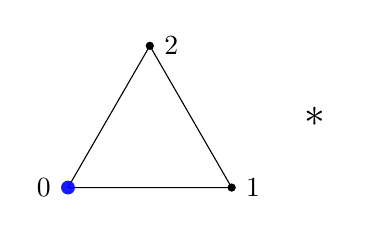
\begin{tikzpicture}[scale=.6]
\coordinate (A) at (210:2);
\coordinate (B) at (-30:2);
\coordinate (C) at (90:2);

\draw[draw=black] (A) -- (B) -- (C) -- (A);

\node[circle,fill=blue, opacity=.9, inner sep=0pt,minimum size=5pt, label=left:{0}] (a) at (A) {};
\node[circle,fill=black,inner sep=0pt,minimum size=3pt, label=right:{$1$}] (a) at (B) {};
\node[circle,fill=black,inner sep=0pt,minimum size=3pt, label=right:{$2$}] (a) at (C) {};

\node[scale=1.5] at (3.5,0.5) {$\ast$};
\end{tikzpicture}
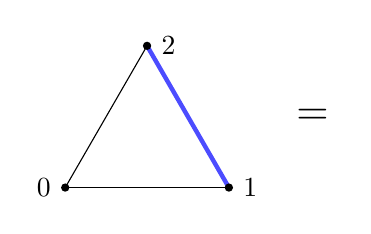
\begin{tikzpicture}[scale=.6]
\coordinate (A) at (210:2);
\coordinate (B) at (-30:2);
\coordinate (C) at (90:2);

\draw[draw=blue, ultra thick, draw opacity=.7] (B) -- (C);
\draw[draw=black] (C) -- (A);
\draw[draw=black] (A) -- (B);

\node[circle,fill=black,inner sep=0pt,minimum size=3pt, label=left:{$0$}] (a) at (A) {};
\node[circle,fill=black,inner sep=0pt,minimum size=3pt, label=right:{$1$}] (a) at (B) {};
\node[circle,fill=black,inner sep=0pt,minimum size=3pt, label=right:{$2$}] (a) at (C) {};

\node[scale=1.5] at (3.5,.5) {=};
\end{tikzpicture}
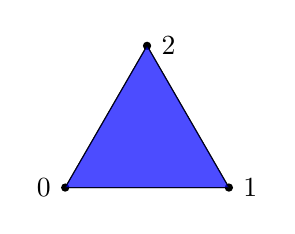
\begin{tikzpicture}[scale=.6]
\coordinate (A) at (210:2);
\coordinate (B) at (-30:2);
\coordinate (C) at (90:2);

\draw[draw=black] (A) -- (B) -- (C) -- (A);

\node[circle,fill=black,inner sep=0pt,minimum size=3pt, label=left:{$0$}] (a) at (A) {};
\node[circle,fill=black,inner sep=0pt,minimum size=3pt, label=right:{$1$}] (a) at (B) {};
\node[circle,fill=black,inner sep=0pt,minimum size=3pt, label=right:{$2$}] (a) at (C) {};

\draw[draw, fill=blue, opacity=.7] (A) -- (B) -- (C) -- (A);
\end{tikzpicture}
	\caption{Geometric representation of the join product of two basis elements. It depicts the identity $\pr \big( [0] \ot [1,2] \big) = [0,1,2]$.}
	\label{f:join of faces}
\end{figure}

\subsection{\texorpdfstring{${E_\infty}$}{E-infty}-coalgebras}

The importance of $\Med$-bialgebras is that they provide a very manageable class of examples of $E_\infty$-coalgebras \cite{medina2020prop1}.
Recall that an $E_\infty$-coalgebra structure on $C$ an operad morphism
\[
\cO \to \coEnd_C
\]
where for $r > 0$ the chain complex $\cO(r)$ is a projective resolution of $\k$ as a (left) $\k[\Sym_r]$-module.